%Revisado

A etapa de preparação de dados é um pilar fundamental em projetos de visão computacional, sendo decisiva para a capacidade de generalização das redes neurais. O objetivo desse processo foi transformar as 3.852 imagens brutas, capturadas no ambiente industrial, em tensores padronizados, isolando a pluma de algodão de qualquer ruído de fundo. 

Para garantir a rastreabilidade, reprodutibilidade e governança do experimento, a arquitetura do \textit{pipeline} de dados foi inspirada no paradigma de medalhas (\textit{Medallion Architecture}), popularizado pela plataforma Databricks \cite{databricks_medallion}. Dessa forma, o fluxo foi estruturado em três estágios lógicos de refinamento: dados brutos e imutáveis (\textit{Bronze}), dados segmentados e padronizados (\textit{Silver}), e tensores finalizados para treinamento (\textit{Gold}).

\subsection{Segmentação Semântica e Remoção de Fundo}

    A primeira transformação aplicada visou isolar estritamente a região de interesse (\textit{Area of Interest} - AOI), removendo as paredes da caixa de captura e a etiqueta amarela de identificação. Para garantir o alinhamento perfeito, a imagem capturada sob iluminação combinada (AB - 2800K e 6000K) foi eleita como referência geométrica para cada amostra (imagem mestre), por oferecer o maior contraste global.

    Em vez de técnicas clássicas de limiarização, que sofrem com as variações de iluminação e sombras inerentes à textura do algodão, optou-se por uma abordagem baseada em aprendizado profundo para a remoção do fundo. Utilizou-se o modelo \textit{BiRefNet} (\textit{Bilateral Reference Network}) \cite{zheng2024birefnet}, uma arquitetura de estado da arte para segmentação dicotômica de imagens. O \textit{BiRefNet} foi escolhido por sua excepcional capacidade de preservar contornos complexos e felpudos, gerando uma máscara binária de alta precisão para a massa de algodão.

    Simultaneamente, para eliminar a etiqueta de rastreabilidade do campo de visão, realizou-se uma segmentação por cor. A imagem foi convertida para o espaço de cores HSV (\textit{Hue, Saturation, Value}), permitindo a criação de uma máscara específica para os tons de amarelo da etiqueta, independentemente da intensidade luminosa. Operações morfológicas de fechamento (\textit{closing}) e dilatação foram aplicadas para garantir a cobertura total da área impressa. Por fim, a máscara da etiqueta foi subtraída da máscara principal do \textit{BiRefNet}, resultando no isolamento puro da pluma de algodão. A evolução visual desse processo de filtragem morfológica, partindo da imagem bruta até a consolidação da máscara final é ilustrada sequencialmente nas Figuras \ref{fig:pipeline_completo}a até \ref{fig:pipeline_completo}d.

\subsection{Cálculo do Maior Retângulo Interno (\textit{Largest Interior Rectangle})}

    Com a pluma isolada, o passo seguinte foi realizar o corte. O uso de uma caixa delimitadora tradicional (\textit{Bounding Box}) foi descartado, pois as bordas orgânicas da amostra fariam com que pixels pretos (do fundo já removido) fossem incluídos no corte, introduzindo ruído no treinamento.

    Para solucionar esse problema, empregou-se o algoritmo do maior retângulo interno (\textit{Largest Interior Rectangle} - LIR). Dado um polígono irregular $\mathcal{P}$ (o contorno da máscara do algodão), o LIR busca encontrar o retângulo $\mathcal{R}$ de área máxima que esteja estritamente contido dentro de $\mathcal{P}$, tal que $\mathcal{R} \subseteq \mathcal{P}$. Esse é um problema clássico de geometria computacional, resolvido por meio da busca do maior sub-histograma em matrizes binárias. 
    
    As coordenadas retangulares $(x_{min}, y_{min}, x_{max}, y_{max})$ obtidas pelo LIR na imagem mestre definiram a AOI definitiva, conforme demonstrado nas Figuras \ref{fig:pipeline_completo}e e \ref{fig:pipeline_completo}f. Essa mesma janela de corte foi então aplicada de forma determinística às imagens correspondentes sob luz quente (AM) e luz fria (BR). Isso garantiu que, para uma mesma amostra física, as três variações de iluminação possuíssem uma amostragem de pixels espacialmente idêntica.

\subsection{Recorte em Blocos e Estruturação do Conjunto de Dados Final}

    Arquiteturas modernas de redes neurais convolucionais e \textit{transformers} tipicamente exigem tensores de entrada quadrados e de dimensões fixas. Como as AOIs geradas pelo LIR possuíam dimensões variadas e resoluções superiores às suportadas pelas redes, adotou-se a estratégia de recorte em blocos.

    Cada recorte retangular foi subdividido em múltiplos \textit{patches} quadrados de $256 \times 256$ pixels. Para evitar a perda de informações nas bordas e nas transições de textura, implementou-se uma taxa de sobreposição (\textit{overlap}) entre os \textit{patches} adjacentes. Essa técnica, além de garantir a cobertura integral da AOI, atua como uma forma robusta de aumento de dados (\textit{Data Augmentation}), multiplicando significativamente o volume do conjunto de treinamento e expondo o modelo a uma maior variabilidade de microtexturas locais da fibra.

    Ao final desse processo, os \textit{patches} foram convertidos para matrizes numéricas e vinculados de volta ao seu \textit{ground truth} (a classe de qualidade oficial obtida no laboratório). Os dados foram então particionados de forma estratificada nos subconjuntos de treinamento, validação e teste, formatados de acordo com os padrões dos \textit{DataLoaders} do \textit{framework} PyTorch, consolidando um conjunto de dados otimizado e pronto para a experimentação arquitetural.


    \begin{figure}[H]
        \centering
        % Linha 1
        \begin{subfigure}[b]{0.32\textwidth}
            \centering
            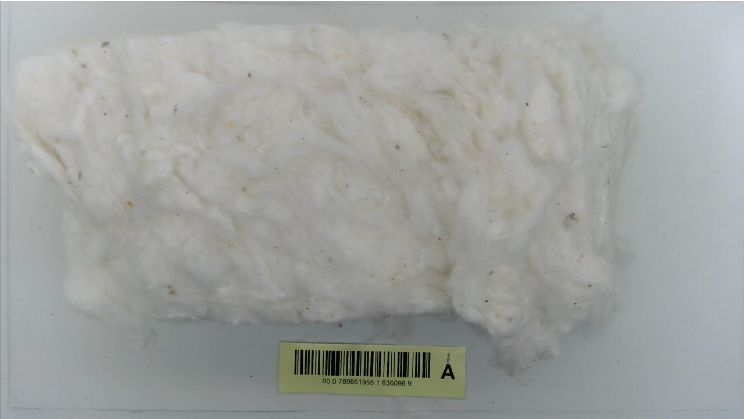
\includegraphics[width=\textwidth]{images/1_amostra_original.pdf}
            \caption{Imagem Bruta (Original)}
            \label{fig:pipe_a}
        \end{subfigure}
        \hfill
        \begin{subfigure}[b]{0.32\textwidth}
            \centering
            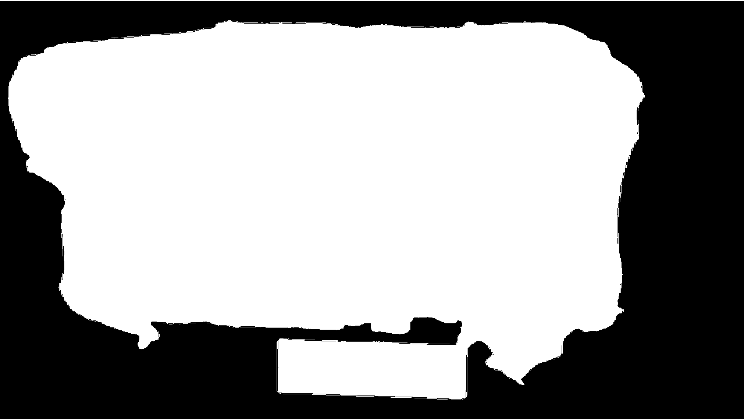
\includegraphics[width=\textwidth]{images/3_mascara_sem_fundo.pdf}
            \caption{Máscara BiRefNet}
            \label{fig:pipe_b}
        \end{subfigure}
        \hfill
        \begin{subfigure}[b]{0.32\textwidth}
            \centering
            
\includegraphics[width=\textwidth]{images/5_mascara_amarelo.pdf}
            \caption{Máscara da Etiqueta (HSV)}
            \label{fig:pipe_c}
        \end{subfigure}
        
        \vspace{0.4cm} % Espaço entre as linhas
        
        % Linha 2
        \begin{subfigure}[b]{0.32\textwidth}
            \centering
            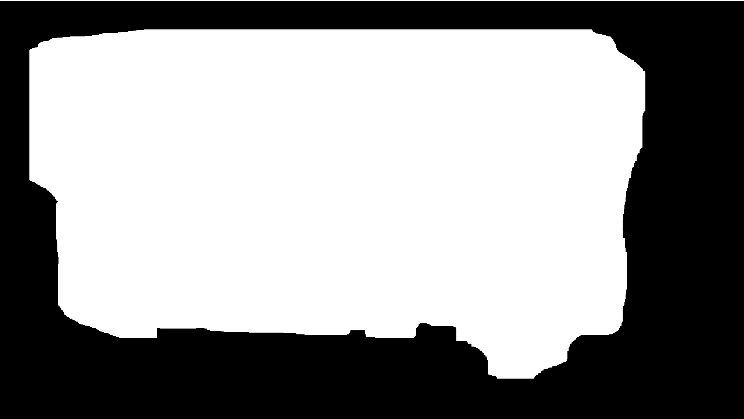
\includegraphics[width=\textwidth]{images/7_mascara_final.pdf}
            \caption{Máscara Final (Subtração)}
            \label{fig:pipe_d}
        \end{subfigure}
        \hfill
        \begin{subfigure}[b]{0.32\textwidth}
            \centering
            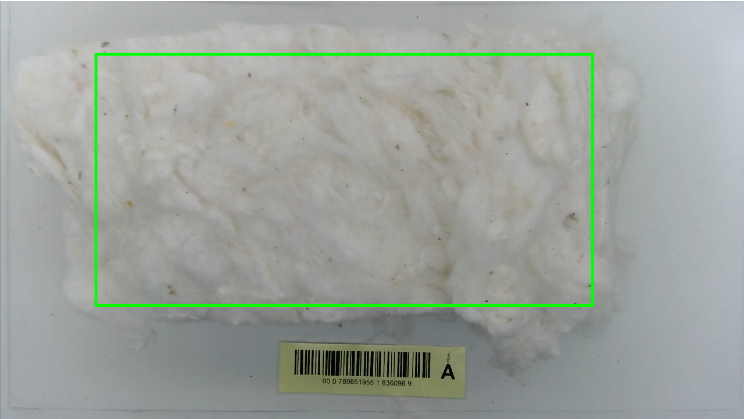
\includegraphics[width=\textwidth]{images/8_retangulo_final.pdf}
            \caption{Maior Retângulo Interno (LIR)}
            \label{fig:pipe_e}
        \end{subfigure}
        \hfill
        \begin{subfigure}[b]{0.32\textwidth}
            \centering
            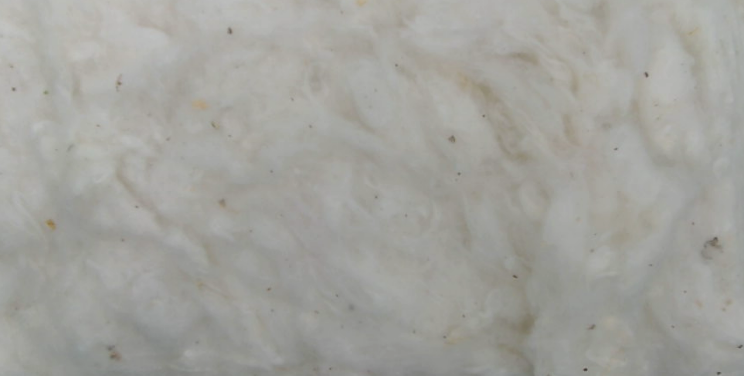
\includegraphics[width=\textwidth]{images/9_imagem_recortada.pdf}
            \caption{Recorte Final (AOI)}
            \label{fig:pipe_f}
        \end{subfigure}
        
        \caption{Etapas sequenciais do \textit{pipeline} de pré-processamento visual: segmentação semântica, operações morfológicas para exclusão de ruídos e definição geométrica da Região de Interesse (AOI).}
        \label{fig:pipeline_completo}
    \end{figure}

\subsection{Engenharia de Características e Expansão Espectral}

    Para avaliar se a injeção de atributos morfológicos pré-computados favorece o desempenho das redes frente ao aprendizado puramente \textit{end-to-end} sobre as matrizes RGB (\textit{Red, Green, Blue}) originais, implementou-se uma ramificação paralela no \textit{pipeline} de pré-processamento. O objetivo foi aplicar a engenharia de características (\textit{feature engineering}) para a extração em multiescala das microtexturas da pluma de algodão.

    A técnica empregada baseou-se em bancos de filtros de Gabor bidimensionais. Por consistirem em funções Gaussianas moduladas por ondas senoidais, esses filtros são matematicamente eficientes para destacar estrias longitudinais, nós de fibras e bordas de micro-impurezas sob diversas perspectivas.

    Para a expansão dos dados, projetou-se um banco contendo 12 \textit{kernels} distintos, gerados pela permutação ortogonal de três frequências espaciais ($f \in \{0,05; 0,10; 0,20\}$) e quatro orientações angulares ($\theta \in \{0^\circ, 45^\circ, 90^\circ, 135^\circ\}$), mantendo-se uma largura de banda (\textit{bandwidth}) constante e ajustada em 0,7. O canal de luminância de cada recorte (\textit{patch}) original foi convoluído com esses filtros. Em seguida, os 12 mapas de magnitude gerados foram empilhados em profundidade com os 3 canais RGB originais, transformando o dado em um tensor morfologicamente enriquecido de 15 canais. Esse conjunto de dados expandido foi salvo de forma isolada, servindo como matriz de entrada alternativa para os ensaios de viabilidade espectral.